\subsection{Initial Documentation}
\subsubsection{Initial Specification}
\begin{figure}[H]
  \centering
  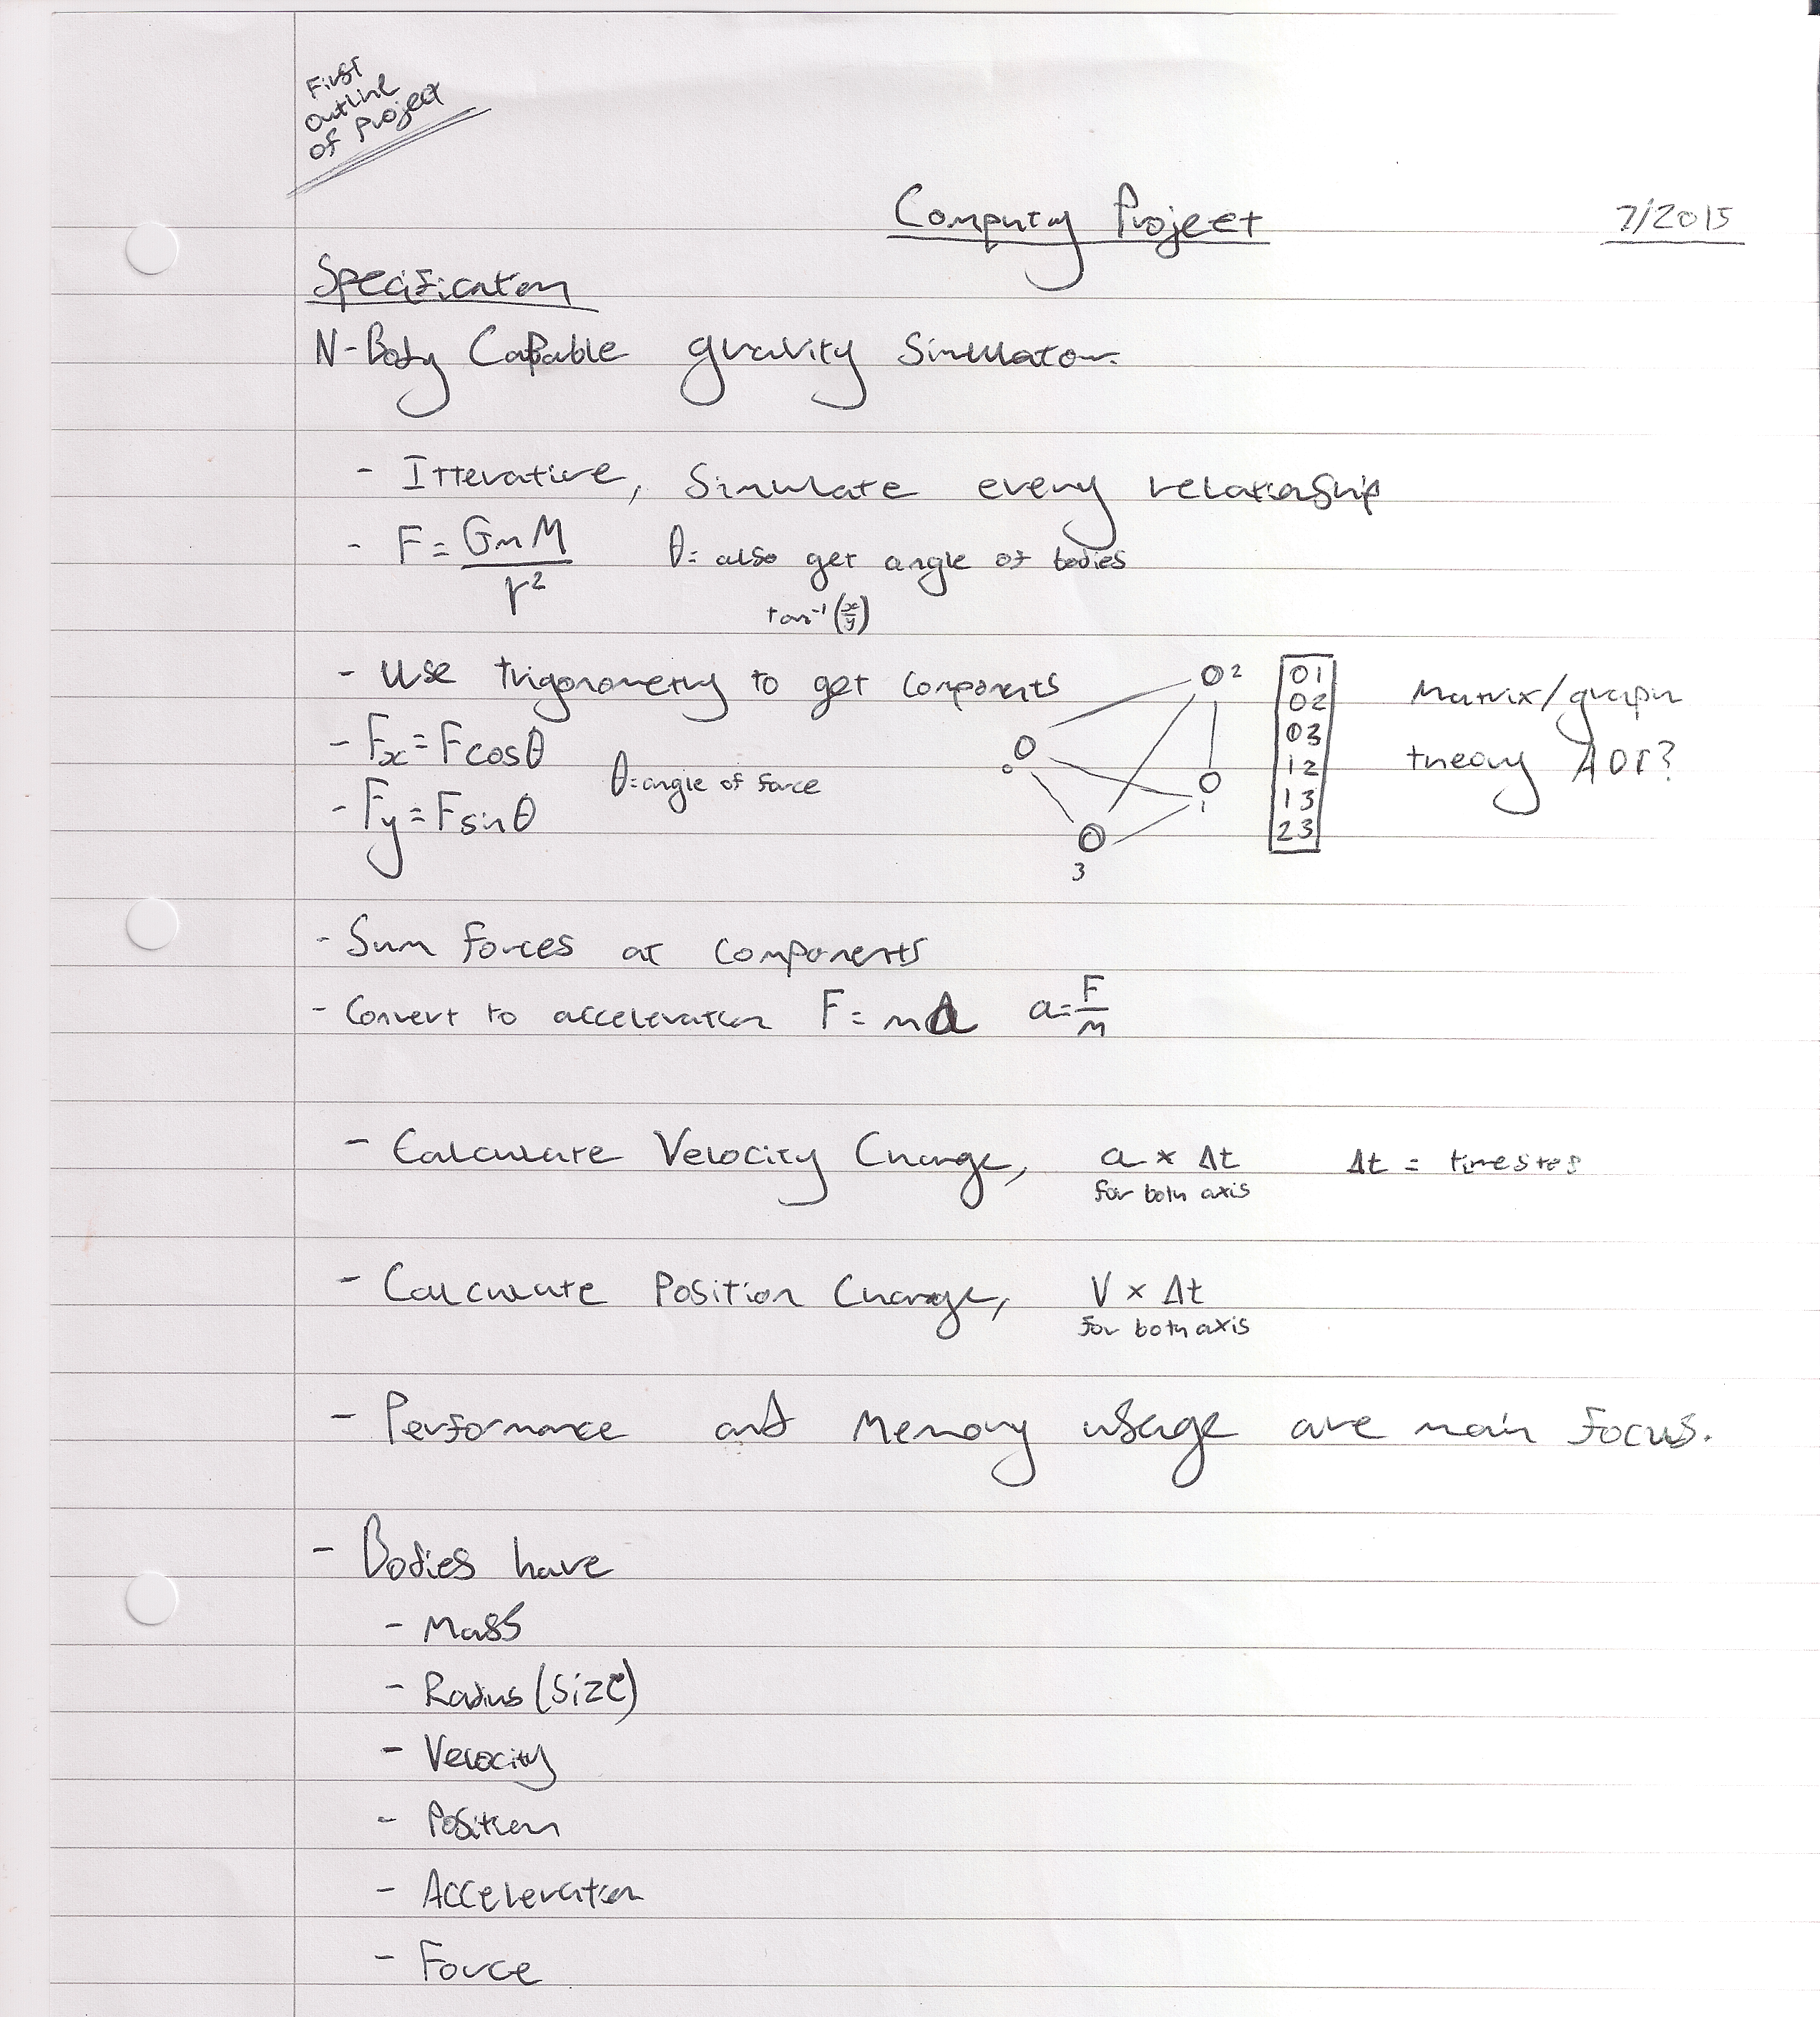
\includegraphics[width=\textwidth]{img/initspec.png}
\end{figure}

\subsubsection{Initial Observation}
\begin{figure}[H]
  \centering
  \includegraphics[width=\textwidth]{img/obs.png}
\end{figure}

\pagebreak

\subsection{Dialogue}
\paragraph{}
I had several brief conversations with my teacher that were not documented during pre-planning stages of the project, these conversations consisted of outlining the idea for a teaching tool that could simulate a scenario set-up by a teacher in order to accurately demonstrate the fundamentals of circular and orbital motion, as a physics student I already have some understanding of what would be required from a project like this.

\begin{small}
\import{sections/appendix/}{dialogue.tex}
\end{small}

